%% LyX 2.0.3 created this file.  For more info, see http://www.lyx.org/.
%% Do not edit unless you really know what you are doing.
\documentclass[english]{article}
\usepackage[T1]{fontenc}
\usepackage[latin9]{inputenc}
\usepackage{graphicx}
\usepackage{babel}
\begin{document}
\begin{center}
General Architecture of the System
\par\end{center}

\begin{figure}
\begin{centering}
\caption{General Architecure of the system}

\par\end{centering}



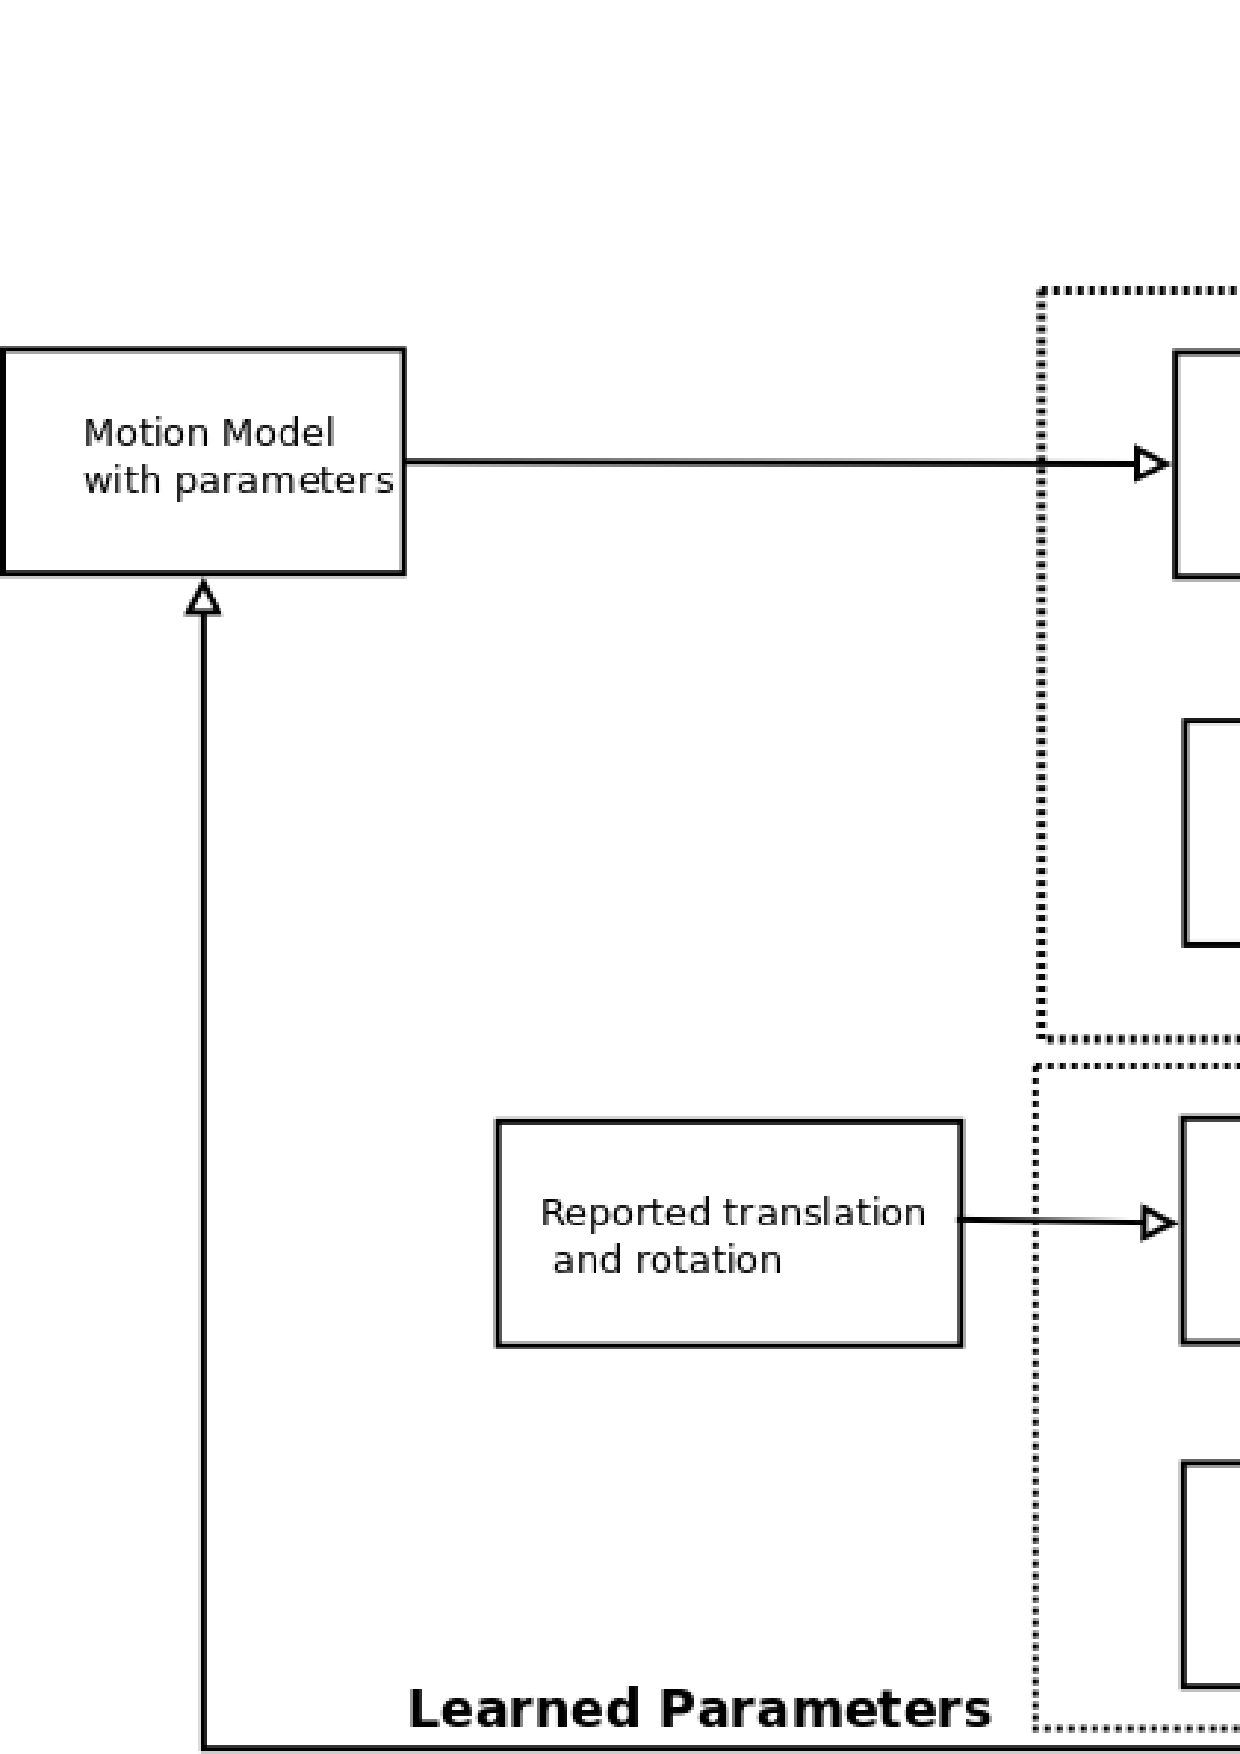
\includegraphics[bb=0bp 0bp 500bp 497bp,scale=0.25]{Diagram1.jpeg}
\end{figure}


The above figure is a block diagram descrubing the whole system. The
first step is to initalize the motion model with a set of parameters.
Then the motion model is used to perform partcile filtering which
is described in detail in the next chapter. The output of this step
is a set of particles with their importance weights.Particle smoothing
is performed on these set of particles. This gives us a collection
of trajectories and completes the Expectation step. 

Based on the trajectories and the reported translational and rotational
motion we calcualte errors at each time step. We perfom newton conjugate
gradient on the errors to give us the best estimate of the paramters.
This compeletes the Maximization Step.

The learned paramters are assigned to the motion model and the whole
process is repeated at each timestep. The whole algorithm gives us
a model which can adapt to dynamic envrioment. The adaptive motion
model perfoms better than the static and the results are shown in
the later chapters.
\end{document}
